\documentclass[border=5pt]{standalone}
\usepackage{xcolor}
\usepackage{pgfplots}
\usepackage{tikz}

% Define bar chart colors
%
\definecolor{bblue}{HTML}{4F81BD}
\definecolor{rred}{HTML}{C0504D}
\definecolor{ggreen}{HTML}{9BBB59}
\definecolor{ppurple}{HTML}{9F4C7C}
\definecolor{orange}{HTML}{FF7E00}
\definecolor{yellow}{HTML}{FFFF66}

\pgfplotsset{every tick label/.append style={font=\large}}

\begin{document}
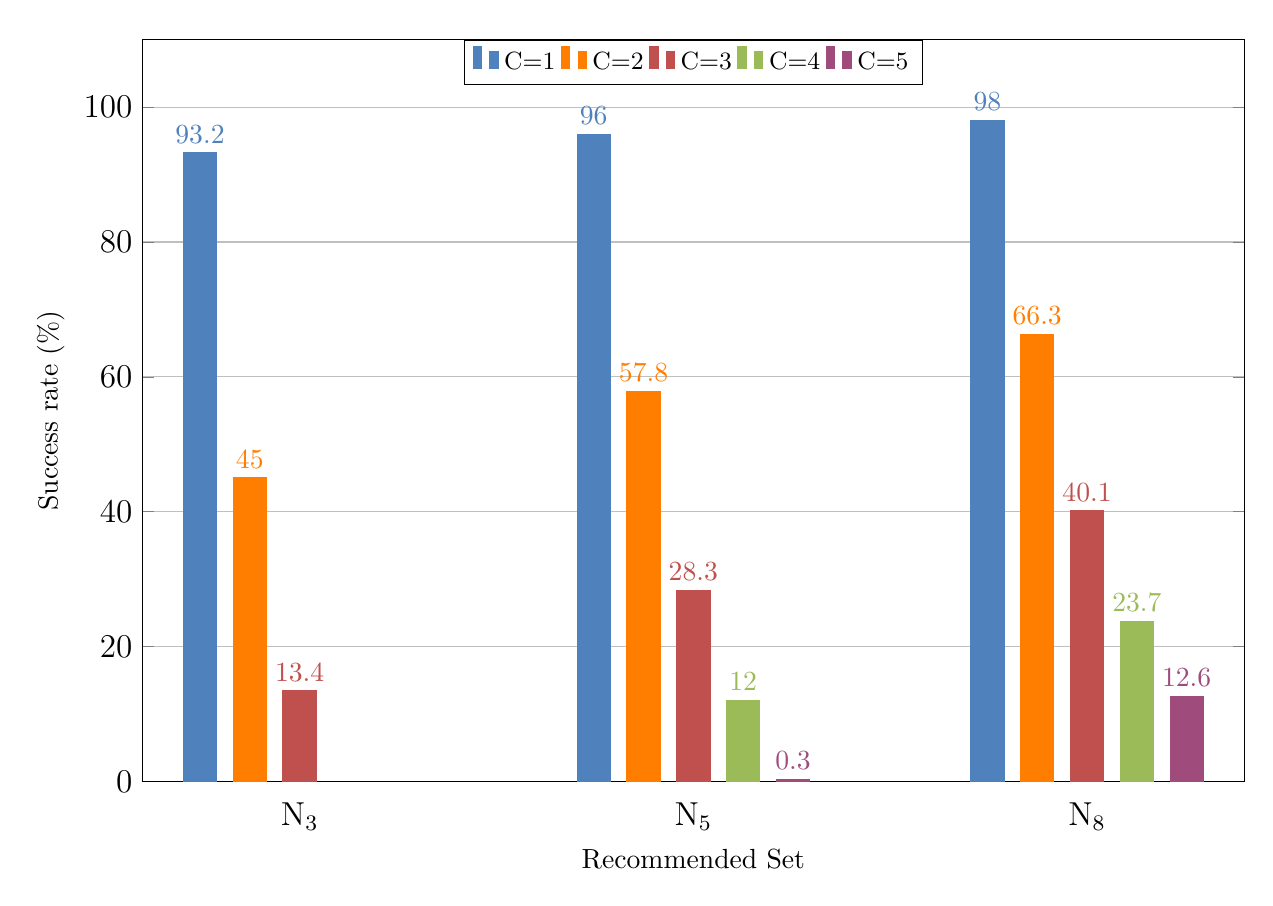
\begin{tikzpicture}
    \begin{axis}[
        width  = 6cm,%*\textwidth,
        height = 11cm,
        major x tick style = transparent,
        ybar = 6pt,
        ymin = 0, ymax = 110,
        x=5cm,
        bar width=12pt,
        ymajorgrids = true,	
        xtick = data,
        scaled y ticks = false,
%		legend style={at={(0.5,-0.1)},
%		legend style={at={(0.5,1.1)}, anchor=north,legend columns=-1,font=\small},
      	legend style={at={(0.5,1)},	anchor=north,legend columns=-1,font=\small,
		anchor=north,legend columns=-1},
		enlarge x limits={abs=2.0cm},
		nodes near coords,
	    xlabel={Recommended Set},
	    ylabel = {Success rate (\%)},
        symbolic x coords={N$_3$,N$_5$,N$_8$},
    ]
%\addplot [style = {fill=aurora}] coordinates {(N:3,93.2) (N:5,96.0) (N:8,98.0)};
%\addplot [style = {fill=hierarch}] coordinates {(N:3,45.0) (N:5,57.8) (N:8,66.3)};
%\addplot [style = {fill=lucene23}] coordinates {(N:3,13.4)(N:5,28.3)(N:8,40.1)};
%\addplot  coordinates {(N:5,12.0)(N:8,23.7)};
%\addplot  coordinates {(N:5,0.3)(N:8,12.6)};    
    
        \addplot[style={bblue,fill=bblue,mark=none}]
            coordinates {(N$_3$, 93.2) (N$_5$,96.0) (N$_8$,98.0)};
            
        \addplot[style={orange,fill=orange,mark=none}]
            coordinates {(N$_3$, 45.0) (N$_5$,57.8) (N$_8$,66.3)};
                      
        \addplot[style={rred,fill=rred,mark=none}]
            coordinates {(N$_3$,13.4) (N$_5$,28.3) (N$_8$,40.1)};

        \addplot[style={ggreen,fill=ggreen,mark=none}]
            coordinates { (N$_5$,12.0) (N$_8$, 23.7)};

        \addplot[style={ppurple,fill=ppurple,mark=none}]
            coordinates { (N$_5$,0.3) (N$_8$,12.6)};

%      	\addplot[style={orange,fill=orange,mark=none}]
%            coordinates {(D$_1$,0.02) (D$_2$,0.902884311) (D$_3$,2.392886747)};


        \legend{C=1, C=2, C=3, C=4, C=5}
    \end{axis}
\end{tikzpicture}
\end{document}